\documentclass[12pt,aspectratio=169]{beamer}

\usetheme[
    sectionpage=progressbar,
    subsectionpage=progressbar,
    progressbar=frametitle
]{metropolis}

\usefonttheme{professionalfonts}

\definecolor{blue-grey-900}{HTML}{263238}
\definecolor{deep-orange-500}{HTML}{FF5722}
\setbeamercolor{normal text}{fg=blue-grey-900, bg=white}
\setbeamercolor{alerted text}{fg=deep-orange-500}

\usepackage{booktabs}
\usepackage{graphicx}
\usepackage{hyphenat}
\usepackage{multirow}

\usepackage{polyglossia}
\setdefaultlanguage[variant=british]{english}
\usepackage[english=british]{csquotes}

\usepackage{fontspec}
\setmainfont{Lucida Sans OT}
\setsansfont[Scale=MatchLowercase]{Lucida Sans OT}
\setmonofont[Scale=MatchLowercase]{Lucida Console DK}
\defaultfontfeatures{Ligatures=TeX}

\usepackage{mathspec}
\setmathsfont(Digits,Latin,Greek)[Numbers={Lining,Proportional}]{Lucida Bright Math OT}

\title{Getting to grips with Databricks}
\author{Gianluca Campanella}
\date{}

\begin{document}

\maketitle

\begin{frame}{Contents}
    \tableofcontents[hideallsubsections]
\end{frame}

\section{Databricks and Spark}

\begin{frame}{What is Databricks?}
    \begin{columns}[b]
        \begin{column}{0.5\textwidth}
            \vfill
            \begin{center}
                
\includegraphics[width=5em]{figures/spark}
            \end{center}
            \vfill
            \begin{itemize}
                \item Cluster computing system
                \item Java, Python, R, Scala and SQL
                \item Apache License 2.0
            \end{itemize}
        \end{column}
        \begin{column}{0.5\textwidth}
            \vfill
            \begin{center}
                
\includegraphics[width=10em]{figures/databricks}
            \end{center}
            \vfill
            \begin{itemize}
                \item Spark as\hyp{}a\hyp{}service
                \item Notebook\hyp{}oriented
                \item Available on Azure and AWS
            \end{itemize}
        \end{column}
    \end{columns}
\end{frame}

\begin{frame}{What is Spark?}
    \begin{columns}
        \begin{column}{0.4\textwidth}
            Spark is\ldots
            \begin{itemize}
                \item Scalable
                \item Fast (\textit{ish})
                \item Simple (\textit{ish})
            \end{itemize}
        \end{column}
        \begin{column}{0.6\textwidth}
            \begin{center}
                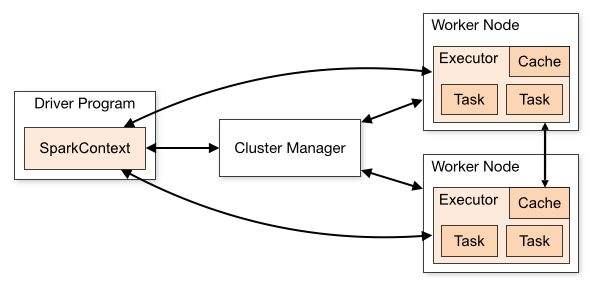
\includegraphics[width=\textwidth]{figures/spark-components} \\
                {\scriptsize%
                 From the Spark documentation}
            \end{center}
        \end{column}
    \end{columns}
\end{frame}

\begin{frame}{Spark use cases}
    \centering
    \begin{tabular}{ll}
        \toprule
        \textbf{Library} & \textbf{Use case}                            \\
        \midrule
        Spark SQL        & Read and process \emph{huge} data sets (ETL) \\
        Spark Streaming  & Process streaming data                       \\
        MLlib            & Train and (batch) score ML models            \\
        GraphX           & Analyse large graphs                         \\
        \bottomrule
    \end{tabular}
\end{frame}

\begin{frame}{Spark DataFrames}
    \begin{itemize}
        \setlength{\itemsep}{\bigskipamount}%
        \item Functionally similar to \texttt{pandas} and R DataFrames
        \item Backed by Resilient Distributed Datasets (RDDs)
        \item Typed ($\to$ querying can be optimised)
    \end{itemize}
\end{frame}

\section{Building E2E solutions}

\begin{frame}{Data Science workflow}
    \begin{center}
        \large%
        Business problem $\ \longleftrightarrow\ $ Research question
        \vfill
        $\updownarrow$
        \vfill
        Obtain $\ \longleftrightarrow\ $ Explore $\ \longleftrightarrow\ $ Model
        \vfill
        $\updownarrow$
        \vfill
        Operationalise
    \end{center}
\end{frame}

\begin{frame}{Running example}
    
\includegraphics[height=2ex]{figures/movielens}
    \begin{block}{`Latest' dataset (9/2018)}
        \begin{itemize}
            \item $5.8 \times 10^{4}$ movies
            \item $2.8 \times 10^{5}$ users
            \item $2.7 \times 10^{7}$ ratings
        \end{itemize}
    \end{block}
\end{frame}

\begin{frame}{Steps}
    \begin{enumerate}
        \setlength{\itemsep}{\bigskipamount}%
        \item Download data
        \item ETL
        \item EDA
        \item Modelling
    \end{enumerate}
\end{frame}

\end{document}
